Find the equation of line 
\begin{enumerate}[label=\thesubsection.\arabic*, ref=\thesubsection.\theenumi]
	\item passing through the point $\vec{P} = (– 4,  3)$ with slope $\frac{1}{2}$.
\label{chapters/11/10/2/2}
\\
\solution
\begin{align}
	\myvec{3&-4}\vec{x}=\myvec{3&-4}\myvec{-2\\3}
	=-18 
\end{align}
is the required equation of the line.

	\item passing through $\myvec{0\\0}$ with slope $m$.\\
\label{chapters/11/10/2/3}
\solution
\begin{align}
	\myvec{3&-4}\vec{x}=\myvec{3&-4}\myvec{-2\\3}
	=-18 
\end{align}
is the required equation of the line.

    \item passing through 
    $\vec{A} = \myvec{2\\2\sqrt{3}}$ and inclined with the x-axis at an angle 
    of 75\degree.
\label{chapters/11/10/2/4}
\\
    \solution 
\begin{align}
	\myvec{3&-4}\vec{x}=\myvec{3&-4}\myvec{-2\\3}
	=-18 
\end{align}
is the required equation of the line.

\item intersecting the x-axis at a distance of 3 units to the left of origin with slope of -2.
\label{chapters/11/10/2/5}
\\
\solution 
\begin{align}
	\myvec{3&-4}\vec{x}=\myvec{3&-4}\myvec{-2\\3}
	=-18 
\end{align}
is the required equation of the line.

\item intersecting the y-axis at a distance of 2 units above the origin and making an
angle of $30\degree$ with positive direction of the x-axis.
\\
\solution 
\begin{align}
	\myvec{3&-4}\vec{x}=\myvec{3&-4}\myvec{-2\\3}
	=-18 
\end{align}
is the required equation of the line.

\item passing through (1, 2) and making angle $30\degree$ with $y$-axis.
\item passing through the points $\vec{A}\myvec{-1\\1}$ and $\vec{B}\myvec{2\\-4}$.
\label{chapters/11/10/2/7}
\\
\solution 
\begin{align}
	\myvec{3&-4}\vec{x}=\myvec{3&-4}\myvec{-2\\3}
	=-18 
\end{align}
is the required equation of the line.

\item passing through the points $(3, 4, -7)$ and $(1, -1, 6)$. 
\item The vector equation of the line 
\begin{align*}
	\frac{x-5}{3}=\frac{y+4}{7}=\frac{z-6}{2} 
\end{align*}
is \noindent\rule{2cm}{0.4pt}. 
\item The vector equation of the line 
\begin{align*}
	\frac{x-5}{3}=\frac{y+4}{7}=\frac{z-6}{2}
\end{align*}
 is \noindent\rule{2cm}{0.4pt}.
\item 
The vertices of triangle $PQR$ are $\vec{P}(2, 1),  \vec{Q}(-2, 3),  \vec{R}(4, 5)$. Find the equation of the median through $\vec{R}$.
\label{chapters/11/10/2/9}
\\
\solution
\begin{align}
	\myvec{3&-4}\vec{x}=\myvec{3&-4}\myvec{-2\\3}
	=-18 
\end{align}
is the required equation of the line.

	\item Find the equations of the planes that pass through the points
\begin{enumerate}
\item $\vec{A}= \myvec{1\\1\\– 1},  \vec{B}=\myvec{6\\4\\– 5}, \vec{C}= \myvec{– 4\\– 2\\3}$
\item $\vec{A}= \myvec{1\\1\\0},  \vec{B}= \myvec{1\\2\\1},  \vec{C}= \myvec{– 2\\2\\-1}$
\end{enumerate}
    \solution
		\begin{enumerate}[label=\thesubsection.\arabic*.,ref=\thesubsection.\theenumi]
	\item 
The intersection of the planes is given as
\begin{align}
	\label{eq:12/11/3/9/input}
\vec{n}_1^{\top}{\vec{x}} - {c}_1 + k\brak{\vec{n}_2^{\top}{\vec{x}} - {c}_2} &= 0
 \vec{n}_1 = \myvec{3\\-1\\2},\,
 \vec{n}_1 = \myvec{1\\1\\1},\,
	c_1 = 4, c_2 = 2.
\end{align}
\begin{align}
	\label{eq:12/11/3/9/eq}
\vec{n}_1^{\top}{\vec{x}} - {c}_1 + \lambda\brak{\vec{n}_2^{\top}{\vec{x}} - {c}_2} &= 0
\end{align}
where 
\begin{align}
	\label{eq:12/11/3/9/lam}
	\lambda = \frac{{c}_1 - \vec{n}_1^{\top}\vec{P}}{\vec{n}_2^{\top}\vec{P} - {c}_2} 
= -\frac{2}{3}  
\end{align}
upon substituting 
\begin{align}
\vec{P} = \myvec{2\\2\\1}.
\end{align}
	in \eqref{eq:12/11/3/9/lam} along with 
the numerical values in 
	\eqref{eq:12/11/3/9/input}.
	Now, substituting
	\eqref{eq:12/11/3/9/lam}
	in \eqref{eq:12/11/3/9/eq},
the equation of plane is 
\begin{align}
 \myvec{7&-5&4}\vec{x} = 8
\end{align}


\end{enumerate}

\item Find the equation of the plane through the points $(2, 1, 0)$,  $(3, -2, -2)$ and $(3, 1, 7)$.
\item A plane passes through the points $(2, 0, 0),  (0, 3, 0)$ and $(0, 0, 4)$. The equation of the plane is \noindent\rule{2cm}{0.4pt}.
\item If the intercept of a line between the coordinate axes is divided by the point (-5, 4) in the ratio 1:2 then find the equation of the line.
\item Find the equation of a line that cuts off equal intercepts on the coordinate axes and passes through the point $(2, 3)$.  
	\\
\solution 
\label{chapters/11/10/2/12}
\begin{align}
	\myvec{3&-4}\vec{x}=\myvec{3&-4}\myvec{-2\\3}
	=-18 
\end{align}
is the required equation of the line.

\item 
Find the equation of a line passing through a point (2, 2) and cutting off intercepts on the axes whose sum is 9.
\label{chapters/11/10/2/13}
	\\
	\solution 
\begin{align}
	\myvec{3&-4}\vec{x}=\myvec{3&-4}\myvec{-2\\3}
	=-18 
\end{align}
is the required equation of the line.

\item Find the equation of the lines which passes the point (3, 4) and cuts off intercepts from the coordinate axes such that their sum is 14.
\item Find the equation of the straight line which passes through the point (1,  -2) and cuts off equal intercepts from axes.
\item Find the equation of the line which passes through the point (-4, 3) and the portion of the line intercepted between the axes is divided internally in ratio 5:3 by this point.
\item Consider the following population and year graph
in \figref{fig:chapters/11/10/1/14/1}.
	Find the slope of the line AB and using it,  find what will be the population in the year 2010.
\\
\begin{figure}[H]
\centering
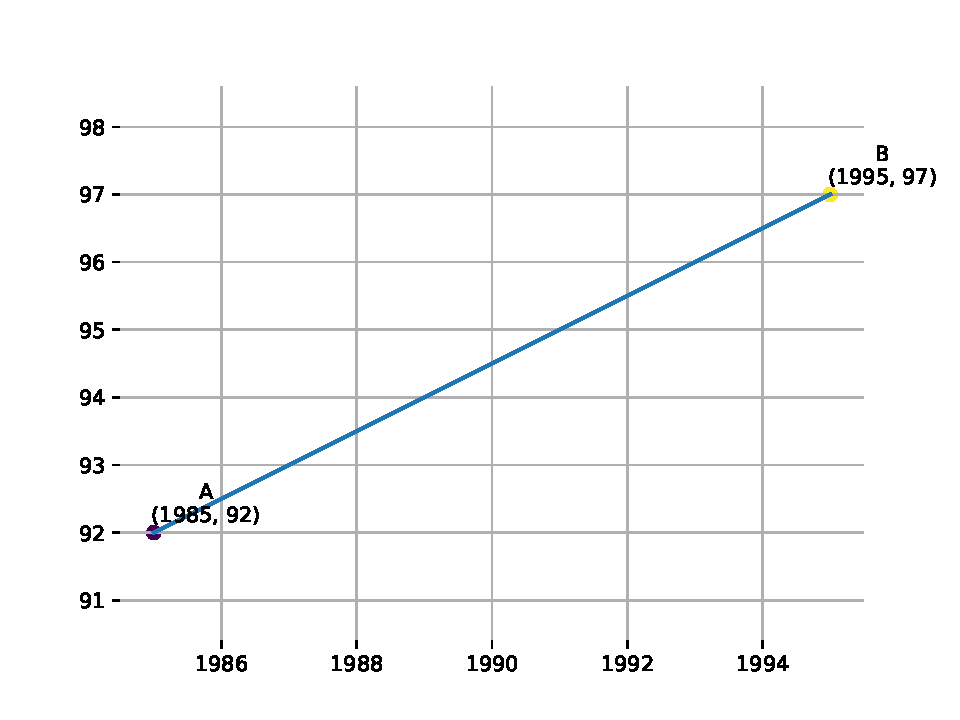
\includegraphics[width=0.75\columnwidth]{chapters/11/10/1/14/figs/fig.pdf}
\caption{}
\label{fig:chapters/11/10/1/14/1}
\end{figure}
\solution
\begin{align}
	\myvec{3&-4}\vec{x}=\myvec{3&-4}\myvec{-2\\3}
	=-18 
\end{align}
is the required equation of the line.

\item Slope of a line which cuts off intercepts of equal length on the axes is 
\begin{enumerate}
\item -1
\item -0
\item 2
\item $\sqrt{3}$
\end{enumerate}
\item If the coordinates of middle point of the portion of a line intercepted between the coordinate axes is (3, 2), then the equation of the line will be
\begin{enumerate}
\item $2x+3y=12$
\item $3x+2y=12$
\item $4x-3y=6$
\item $5x-2y=10$
\end{enumerate}
\item If the line $\frac{x}{a}+\frac{y}{b}=1$ passes the points (2, -3) and (4, -5),  then $(a, b)$ is 
\begin{enumerate}
\item (1, 1)
\item (-1, 1)
\item (1, -1)
\item (-1, -1)
\end{enumerate}
\item The intercepts made by the plane $2x-3y+5z+4=0$ on the co-ordinate axis are $\brak{-2, \frac{4}{3}, -\frac{4}{5}}$.
\item The line $\overrightarrow{r}=2\hat{i}-3\hat{j}-\hat{k}+\lambda(\hat{i}-\hat{j}+2\hat{k})$ lies in the plane $\overrightarrow{r} \cdot (3\hat{i}+\hat{j}-\hat{k})+2=0$.
\item Find the equation of the line joining $(1, 2)$ and $(3, 6)$.
\item Find the equation of the line joining $(3, 1)$ and $(9, 3)$.
\item If the point (3,  4) lies on the line $3y=ax+7$,  find the value of $a$.
\item  Find the equation of the line that passes through the point with position vector $2\hat{i}-\hat{j}+4\hat{k}$ and is in direction $\hat{i}+2\hat{j}-\hat{k}$.
\item The cartesian equation of a line is $ \frac{x-5}{3}=\frac{y+4}{7}=\frac{z-6}{2}$. Write its vector form.
\item Find the equation of the line that passes through the origin and $(5, -2, 3)$.
\item Find the equation of the line that passes through the points $(3, -2, -5), (3, -2, 6)$.
\item Find the coordinates of the point where the line through $(5,1,6)$ and $(3,4,1)$ crosses the $YZ$-plane.
\item Find the coordinates of the point where the line through $(5,1,6)$ and $(3,4,1)$ crosses the $ZX$-plane.
\item Find the coordinates of the point where the line through $(3,-4,-5)$ and $(2,-3,1)$ crosses the plane $2x+y+x=7$.
\item Find the equation of the line through $(-2,3)$ with slope $-4$
\item Write the equation of the line through the points $(1,-1)$ and $(3,5)$.
\item Write the equation of the lines for which $\tan \theta=\frac{1}{2}$, where $\theta$ is the inclination of the line and
\begin{enumerate}
\item  y-intercept is $\frac{-3}{2}$ 
\item  x-intercept is $4$.
\end{enumerate}
\item Find the equation of the lines which makes intercepts $-3$ and $2$ on the x- and y-axes respectively.
\item Equation of a line is $3x-4y+10=0$, Find its
\begin{enumerate}
\item  Slope
\item  x and y-intercepts.
\end{enumerate}
\item The Fahrenheit temperature $F$ and  absolute temperature $K$ satisfy a linear equation. Given that $K=273$ when $F=32$ and that $K=373$ when $F=212$. Express $K$ in terms of $F$ and find the value of $F$, when $K=0$.
\item A line is such that its segment between the lines $5x-y+4=0$ and $3x+4y-4=0$ is bisected at the point $(1,5)$. Obtain its equation.
\item Find the vector equations of the plane passing through the points $R(2, 5, -3), S(-2, -3, 5)$ and $T(5, 3, -3)$.
\item Find the equation of the plane with intercepts $2, 3$ and $4$ on the x, y and z - axis respectively.
\item Show that the lines 
\begin{align}
\frac{x-a+d}{\alpha -\delta} =\frac{y-a}{\alpha} =\frac{z-a-d}{\alpha +\delta}\\
 \text{  and } 
	\\
	\frac{x-a+c}{\beta -\gamma} =\frac{y -b}{\beta} =\frac{z-b-c}{\beta +\gamma} 
\end{align}
 are coplanar.
\item Show that the lines 
\begin{align}
\frac{x+3}{-3}= \frac{y-1}{1}= \frac{z-5}{5} \text{ and } 
	\\
	\frac{x+1}{-1} =\frac{y-2}{2} =\frac{z-5}{5}. 
\end{align}
are coplanar.
\item Find the equation for the line passing through the points $(-1, 0, 2)$ and $(3, 4, 6)$.
\item The Cartesian equation of a line is
\begin{align}
\frac{x+3}{2}= \frac{y-5}{4}= \frac{z+6}{2}
\end{align} 
Find the vector equation for the line.
\item Determine the ratio in which the line $2x+y  - 4=0$ divides the line segment joining the points  $\vec{A}(2, - 2)$  and  $\vec{B}(3, 7)$.
\\
\solution
	The desired vector is
\begin{align}
\frac{1}{2}\myvec{2\\3\\4} +  \frac{1}{2}\myvec{4\\1\\-2} =\myvec{3\\2\\1} 
\end{align}




\item The line segment joining the points $\vec{A}(3,2)$ and $\vec{B}(5,1)$ is divided at the point $\vec{P}$ in the ratio 1:2 which lies on $3x-18y+k=0$. Find the value of $k$.  
\item Find the ratio in which the line $2x+3y-5=0$ divides the line segment joining the points $(8,-9)$ and $(2,1)$. Also find the coordinates of the point of division.
\item Find the ratio in which the $YZ$ plane divides the line segment formed by joining the points $(-2,4,7)$ and $(3,-5,8)$.
\item Find the ratio in which the line segment joining the points $(4,8,10)$ and $(6,10,-8)$ is divided by the $YZ$ plane.
\item Find the ratio in which the $Y$ axis divides the line segment joining the points $(5,-6)$ and $(-1,-4)$. Also find the point of intersection.
\item In what ratio does the $X$ axis divide the line segment joining the points $(-4,-6)$ and $(-1,7)$? Find the coordinates of the point of division.
\item Find the ratio in which the line segment joining $\vec{A}(1,-5)$  and  $\vec{B}(-4,5)$ is divided by the $X$ axis. Also find the coordinates of the point of division.
\item A line intersects the $Y$ axis and $X$ axis at the points $\vec{P}$  and $\vec{Q}$,  respectively. lf $(2, 5)$ is the mid-point of $PQ$,  then the coordinates of $\vec{P}$ and $ \vec{Q}$ are,  respectively
\begin{enumerate}
	\item$(0,-5)$ and $(2,0)$
	\item$(0,-10)$ and $(-4,0)$
	\item$(0,4)$ and  $(-10,0)$
	\item$(0,-10)$ and $(4,0)$
\end{enumerate}
\item Check which of the following are solutions of the equation $x-2y=4$ and which 
are not
\begin{enumerate}
\item ($0, 2$)
\item ($2, 0$)
\item ($4, 0$)
\item ($\sqrt 2,  4\sqrt 2$)
\item ($1, 1$)
\end{enumerate}
\item Equations of the diagonals of the square formed by the lines $x=0$,  $y=0$,  $x=1$ and $y=1$ are

\end{enumerate}
